\documentclass[a4paper,12pt]{article}

% Pakete für Layout und Funktionalität
\usepackage[utf8]{inputenc} % Umlaute
\usepackage[T1]{fontenc} % Schriftkodierung
\usepackage{mathpazo} % Times New Roman für bessere Lesbarkeit
\usepackage[provide=*,ngerman]{babel} % Deutsche Sprache
\usepackage{geometry} % Seitenränder
\geometry{a4paper, margin=2.5cm}

% Absatzabstand konfigurieren
\setlength{\parskip}{0.5\baselineskip} % Halbe Zeile Abstand zwischen Absätzen
\setlength{\parindent}{0pt} % Keine Einrückung am Absatzanfang

\usepackage{graphicx} % Bilder einfügen
\usepackage{hyperref} % Hyperlinks
\usepackage{bookmark} % Verbesserte Unterstützung für Bookmarks und Outlines
\usepackage{titlesec} % Anpassung der Überschriften
\usepackage{booktabs} % Schönere Tabellen
\usepackage{array} % Erweiterte Tabellenoptionen
\usepackage{etoolbox}
\usepackage{fancybox} % Für verschiedene Boxen-Stile
\usepackage{tipa} % Unterstützt IPA-Zeichen
\usepackage{float} % Paket für erzwungene Platzierung von Tabellen
\usepackage{wrapfig} % Für Textumfluss um Boxen

% Titel und Autor
\title{Reiseplanung Skandinavien 2026}
\author{Steffen}
\date{5. Januar 2026}

\begin{document}

% Deckblatt
\maketitle
\begin{center}
    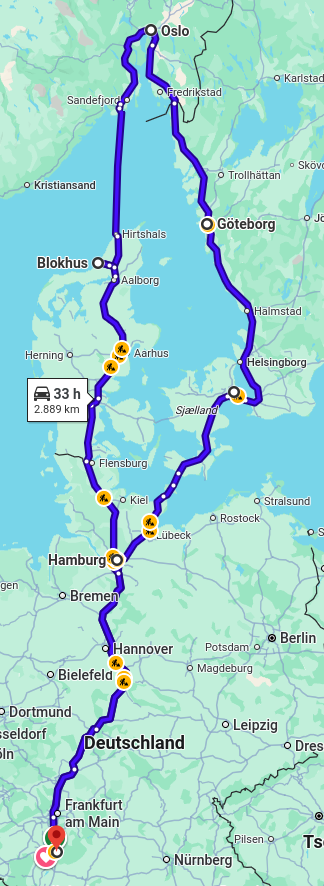
\includegraphics[width=0.4\textwidth]{Reiseroute (Google Maps).png} % Reiseroute Bild eingefügt
\end{center}
\newpage

% Inhaltsverzeichnis
\tableofcontents
\newpage

% Einleitung
\section{Einleitung}
Diese Reiseplanung beschreibt die geplante Reise nach Skandinavien im Jahr 2026. Ziel ist es, die schönsten Orte zu besuchen und eine unvergessliche Zeit zu erleben.

% Reiseroute
%
% Start am 8. August 2026 in 69469 Weinheim, Senecaweg 16
% - Lübeck mit 2 Tagen Übernachtung
% - Kopenhagen mit 2 Tagen Übernachtung
% - Göteborg mit 2 Tagen Übernachtung
% - Blokhus mit 7 Tagen Übernachtung
% Rückreise am 22. August 2026

Wir wollen den Urlaub in Skandinavien in zwei Teile aufteilen: im ersten Teil bereisen wir zwei Länder (Dänemark, Schweden) und im zweiten Teil die Insel im Norden Dänemarks, das Nordjylland.

Der eigentliche Startpunkt ist die Hansestadt Lübeck. Von hier bereisen wir die Städte Kopenhagen und Göteborg. In der Nähe dieser Städte werden wir je zwei- oder dreimal Übernachten, um einen Eindruck von der Gegend zu bekommen und die Städte auch entsprechend zu beischtigen.

Im zweiten Teil der Reise werden wir uns dann in Blockhus, Dänemark, erholen und auf die Erlebnisse des ersten Reiseteils zurückschauen.

Eine Übersicht der Reisedaten findet sich im Abschnitt Reisedaten (\ref{tab:Reisedaten}).

Den überwiegenden Teil der Strecken legen wir mit dem Auto zurück. Die reine Fahrzeit laut Reisedaten beträgt 29h 47min; zusätzlich planen wir Ladestopps von jeweils etwa 30 Minuten pro 350--400 km ein.

Für den Grenzwechsel zwischen Dänemark und Schweden nutzen wir auf der Hinfahrt die Öresundbrücke (E20) von Kopenhagen über Malmö nach Göteborg. Dafür sind Maut-Gebühren zu entrichten.

\textbf{Mautgebühren Öresundbrücke (ab Januar 2026):}
\begin{itemize}
\item Online-Ticket (mit 10\% Rabatt): 420 DKK (ca. 56,30 EUR) pro Einzelfahrt
\item Online-Buchung unter: \url{https://www.oresundsbron.com/tickets}
\end{itemize}

\begin{figure}[H]
    \centering
    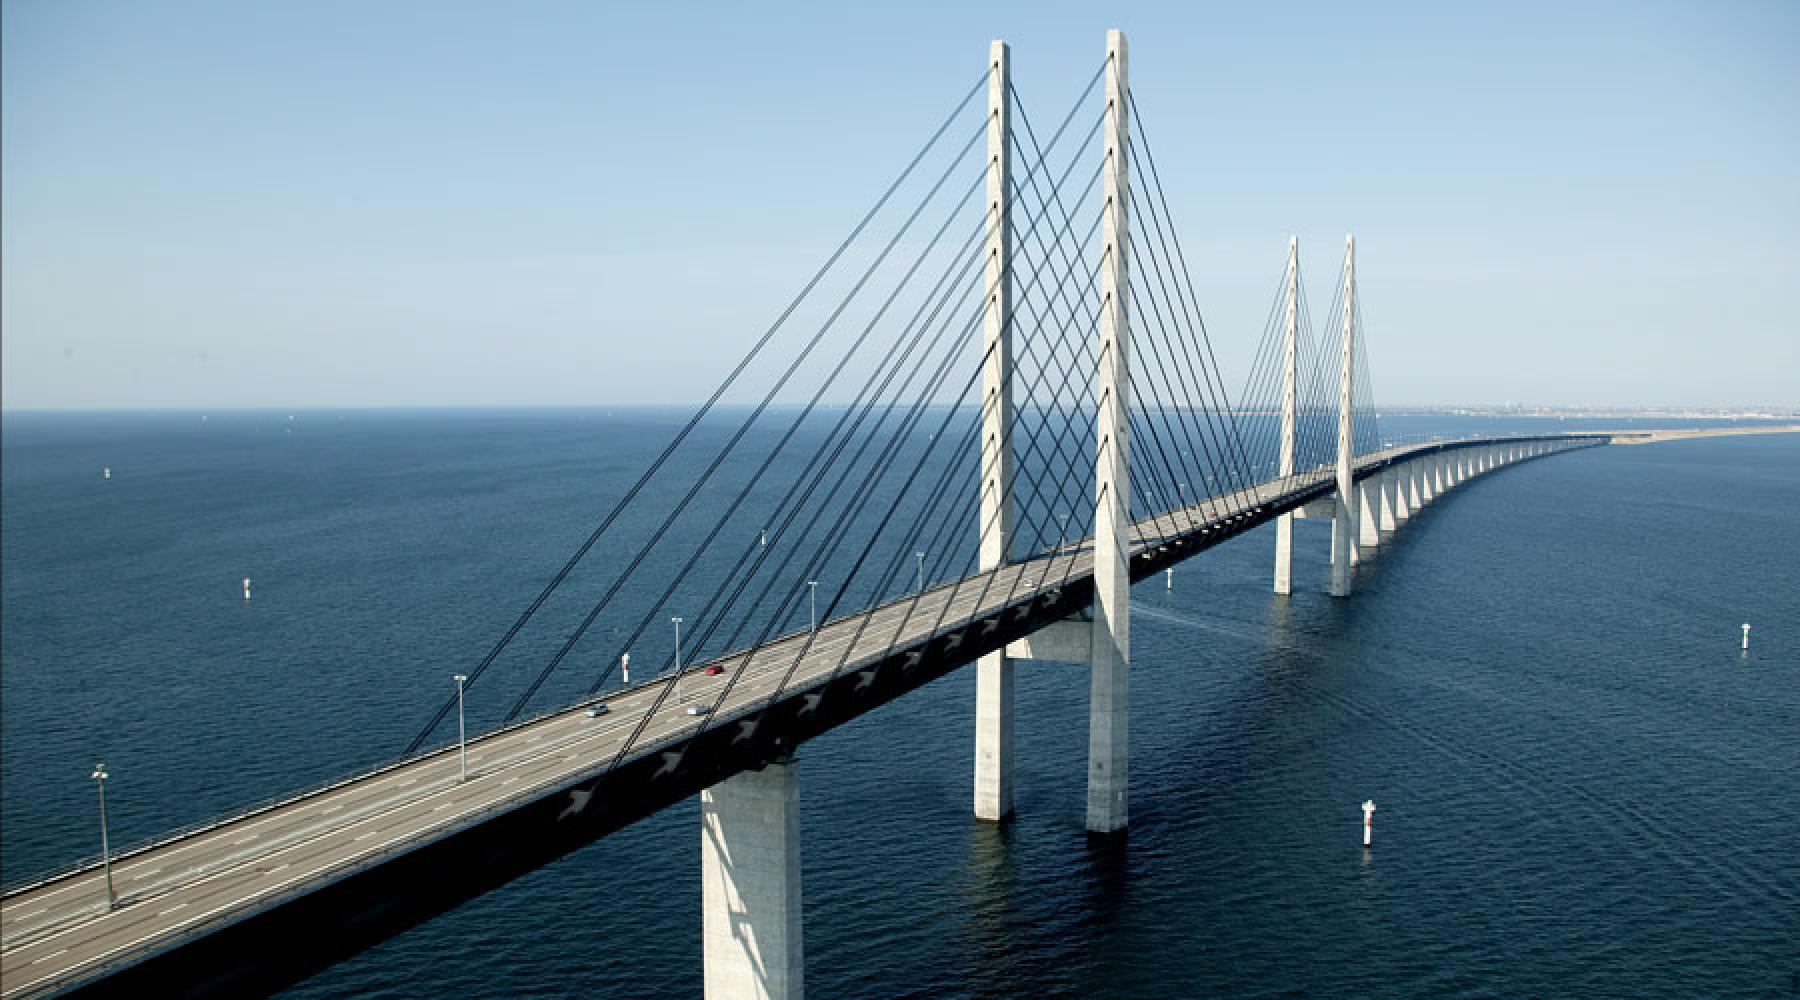
\includegraphics[width=0.72\textwidth]{Oeresundbruecke.jpg} % Bild der Öresundbrücke eingefügt
    \caption{Die Öresundbrücke verbindet Dänemark und Schweden.}
    \label{fig:oeresundbruecke}
\end{figure}

\textbf{Fährverbindung Göteborg $\leftrightarrow$ Frederikshavn (Dänemark):}
\begin{itemize}
\item Reederei: Stena Line mit den Fähren Stena Danica und Stena Jutlandica
\item Fahrtzeit: 3,5 Stunden pro Überfahrt
\item Geplante Verbindung für den 15.08.2026: 09:05--12:35 mit Stena Danica
\item Check-in schließt 30 Minuten vor Abfahrt
\item Preis: ab 697 DKK (ca. 94 EUR) für Einzelfahrt mit PKW und Fahrer
\item Geplanter Tarif: Premium für 199,70 EUR (Kostenlose Umbuchung, 100\% Rückerstattung bis zu 2 Std. vor Abfahrt, Bevorzugtes Boarding, Bevorzugtes Ausschiffen)
\item Buchung online unter: \newline \url{https://www.stenaline.de/routen/frederikshavn-goeteborg}
\end{itemize}


% Reiseziele
\section{Reiseziele}
\subsection{Lübeck, Deutschland}

\begin{wrapfigure}{r}{0.4\textwidth}
\footnotesize
\fbox{%
\parbox{0.35\textwidth}{%
\textbf{Grundlegende Informationen} - Lübeck als Hansestadt mit \mbox{217.000} Einwohnern

\textbf{Historische Bedeutung} - Gründung 1143, Hanse-Hauptstadt im Mittelalter

\textbf{UNESCO-Weltkulturerbe} - Die mittelalterliche Altstadt seit 1987

\textbf{Architektonische Highlights} - Die sieben Türme, Holstentor, Rathaus

\textbf{Besondere Merkmale} - Gänge und Höfe, Lübecker Marzipan

\textbf{Travemünde} - Seebad und Fährhafen nach Skandinavien
}%
}
\end{wrapfigure}

Lübeck ist eine kreisfreie Hansestadt in Schleswig-Holstein mit etwa \mbox{217.000} Einwohnern. Die Stadt wurde 1143 als erste deutsche Hafenstadt an der Ostsee gegründet und war von 1226 bis 1937 ein eigenständiger Stadtstaat. Als Hauptort der Hanse gehörte Lübeck im 13. und 14. Jahrhundert zu den bedeutendsten Städten Nordeuropas.

Die mittelalterliche Altstadt von Lübeck ist seit 1987 UNESCO-Weltkulturerbe und liegt auf einer ovalen Insel zwischen Stadt-Trave und Kanal-Trave. Das Stadtbild wird geprägt durch die sieben charakteristischen Kirchtürme der fünf großen Altstadtkirchen: Marienkirche (mit den höchsten Backsteintürmen der Welt), Dom zu Lübeck, Petrikirche, Jakobikirche und Aegidienkirche.

Zu den wichtigsten Sehenswürdigkeiten gehören das berühmte Holstentor (Wahrzeichen der Stadt), das historische Rathaus mit seiner einzigartigen Backsteinarchitektur und die zahlreichen Lübecker Gänge und Höfe - enge Wohnquartiere, die aus Platznot in den Hinterhöfen entstanden sind.

Lübeck ist weltberühmt für sein Marzipan, das hier seit dem späten Mittelalter hergestellt wird. Die Stadt gilt als „Königin der Hanse" und beeindruckt noch heute mit ihrer nahezu vollständig erhaltenen mittelalterlichen Bausubstanz. Etwa drei Viertel der Gebäude in der Altstadt wurden im Zweiten Weltkrieg nicht zerstört.

Der Stadtteil Travemünde, etwa 17 Kilometer von der Altstadt entfernt, ist ein traditionsreiches Seebad an der Ostsee mit breiten Sandstränden und dient als wichtiger Fährhafen nach Skandinavien.

\subsubsection{Beschreibung der Sehenswürdigkeiten und Aktivitäten}
\begin{itemize}
\item \textbf{Flüchtlingshof, Glandorps Gang und Rosengang}\newline
Kriterium: \textit{Lokal-Favorit, deutlich abseits vom Massentourismus}.\newline
Ort: Altstadt-Innenhöfe rund um Glockengießerstraße/Koberg\newline
Anreise: Sehr gut per Fahrrad erreichbar, anschließend zu Fuß durch die Höfe.\newline
Karte: \url{https://www.google.com/maps/search/?api=1&query=Fuechtingshof+Luebeck}

\item \textbf{Hospital zum Heiligen Geist}\newline
Kriterium: \textit{Lokal plus Kultur, weniger Mainstream als die klassischen Fotospots}.\newline
Ort: Koberg 11, 23552 Lübeck\newline
Anreise: Zentral in der Altstadt, gut zu Fuß oder per Fahrrad.\newline
Karte: \url{https://www.google.com/maps/search/?api=1&query=Hospital+zum+Heiligen+Geist+Luebeck}

\item \textbf{Drägerpark}\newline
Kriterium: \textit{Wenig Mainstream, lokale Grün-Oase}.\newline
Ort: Wakenitzufer, St.-Jürgen, Lübeck\newline
Anreise: Mit Fahrrad gut erreichbar, ruhigere Alternative zur Altstadt.\newline
Karte: \url{https://www.google.com/maps/search/?api=1&query=Draegerpark+Luebeck}

\item \textbf{Burgtor}\newline
Kriterium: \textit{Historisch relevant, meist weniger überlaufen als Holstentor}.\newline
Ort: Große Burgstraße, Lübeck\newline
Anreise: Per Fahrrad oder zu Fuß aus der Altstadt.\newline
Karte: \url{https://www.google.com/maps/search/?api=1&query=Burgtor+Luebeck}

\item \textbf{Travemünde als ruhiger Außenpunkt}\newline
Kriterium: \textit{Lokale Küstenatmosphäre außerhalb der Kern-Altstadt}.\newline
Ort: Travemünde, Lübeck\newline
Anreise: Am besten per Auto oder mit ÖPNV/Fahrrad als Halbtagesausflug.\newline
Karte: \url{https://www.google.com/maps/search/?api=1&query=Travemuende+Luebeck}
\end{itemize}

\subsubsection{Kulinarische Empfehlungen (mittleres Budget)}
\begin{itemize}
\item \textbf{Restaurant Schiffergesellschaft} -- Ausgewählt wegen hanseatischer Tradition, norddeutscher Küche und guter Mischung aus lokalem Publikum und Besuchern. Für Lübeck ein Klassiker mit viel Charakter.\newline
Adresse: Breite Straße 2, 23552 Lübeck\newline
Kontakt/Reservierung: +49 451 76 776, \url{https://www.schiffergesellschaft.de/}\newline
Erreichbarkeit: Gut per Fahrrad aus der Altstadt, alternativ per Auto.

\item \textbf{Backup: Café Niederegger} -- Lübecker Institution mit starker lokaler Prägung; ideal für regionale Konditorei-Spezialitäten, Frühstück oder leichte Mittagszeit im mittleren Budget.\newline
Adresse: Breite Straße 89, 23552 Lübeck\newline
Kontakt/Reservierung: +49 451 53 01 - 126 / 127, \url{https://www.niederegger.de/cafe-niederegger/}\newline
Erreichbarkeit: Zentral und sehr gut per Fahrrad, Parkmöglichkeiten in der Innenstadt mit dem Auto.
\end{itemize}


\subsection{Kopenhagen, Dänemark}
Kopenhagen (dänisch København) ist die Hauptstadt Dänemarks und das kulturelle und wirtschaftliche Zentrum des Landes. Die Stadt ist Sitz von Parlament (Folketing), höchstem Gericht und Regierung. Die dänische Hauptstadt gehört zu den bedeutendsten Metropolen Nordeuropas, ist ein beliebtes Reiseziel und Seehafenstadt. Die Kommune Kopenhagen (Københavns Kommune) hat \mbox{667.099} Einwohner, die Hauptstadt im formalen Sinne (bestehend aus den Kommunen Kopenhagen, Frederiksberg und Gentofte) \mbox{848.015} Einwohner. Kopenhagen ist Teil der dänischen Verwaltungsregion Region Hovedstaden und der binationalen Metropolregion Öresundregion. Die Stadt gilt als eine der Städte mit der größten Lebensqualität weltweit. In der Städteplatzierung des Beratungsunternehmens Mercer belegte sie im Jahr 2024 unter 241 Großstädten weltweit den vierten Platz in dieser Rubrik. In dem von der Economist Group herausgegebenen Global Liveability Index belegte Kopenhagen 2023 Platz 2 der lebenswertesten Städte der Welt.

\subsubsection{Beschreibung der Sehenswürdigkeiten und Aktivitäten}
\begin{itemize}
\item \textbf{Jægersborggade}\newline
Kriterium: \textit{Lokal-Favorit mit Cafés und kleinen Läden, authentischer als die Einkaufsachsen im Zentrum}.\newline
Ort: Nørrebro, Kopenhagen\newline
Anreise: Per Fahrrad oder Metro/S-Bahn plus kurzer Fußweg.\newline
Karte: \url{https://www.google.com/maps/search/?api=1&query=Jaegersborggade+Kopenhagen}

\item \textbf{Superkilen}\newline
Kriterium: \textit{Außergewöhnlicher Stadtpark, wenig klassischer Mainstream}.\newline
Ort: Nørrebro, Kopenhagen\newline
Anreise: Per Fahrrad sehr gut erreichbar.\newline
Karte: \url{https://www.google.com/maps/search/?api=1&query=Superkilen+Kopenhagen}

\item \textbf{Cisternerne}\newline
Kriterium: \textit{Kultur-Spot abseits Standardprogramm}.\newline
Ort: Søndermarken, Frederiksberg\newline
Anreise: Gut per Fahrrad oder Metro/Bus erreichbar.\newline
Karte: \url{https://www.google.com/maps/search/?api=1&query=Cisternerne+Frederiksberg}

\item \textbf{Refshaleøen und Reffen}\newline
Kriterium: \textit{Lokale Wasserkante mit kreativem Quartier und Food-Konzept, deutlich weniger klassisch touristisch}.\newline
Ort: Refshaleøen, Kopenhagen\newline
Anreise: Per Fahrrad sehr gut erreichbar.\newline
Karte: \url{https://www.google.com/maps/search/?api=1&query=Refshaleoen+Kopenhagen}

\item \textbf{Nordhavn}\newline
Kriterium: \textit{Modernes Hafenviertel, jenseits der klassischen Altstadt-Routen}.\newline
Ort: Nordhavn, Kopenhagen\newline
Anreise: Per Fahrrad oder S-Bahn/Metro erreichbar.\newline
Karte: \url{https://www.google.com/maps/search/?api=1&query=Nordhavn+Kopenhagen}

\item \textbf{Louisiana Museum of Modern Art (Ausflug)}\newline
Kriterium: \textit{Hochwertiger Kultur-Ausflug mit Küstenlage, nicht Teil des Massentourismus in der Innenstadt}.\newline
Ort: Gl Strandvej 13, 3050 Humlebæk\newline
Anreise: Regionalzug Richtung Humlebæk, anschließend kurzer Fußweg.\newline
Karte: \url{https://www.google.com/maps/search/?api=1&query=Louisiana+Museum+of+Modern+Art+Humlebaek}
\end{itemize}

\subsubsection{Kulinarische Empfehlungen (mittleres Budget)}
\begin{itemize}
\item \textbf{Restaurant Kronborg} -- Ausgewählt wegen klassischer dänischer Küche (Smørrebrød), starker lokaler Verankerung und guter Preis-Leistung für Kopenhagen.\newline
Adresse: Brolæggerstræde 12, 1211 København K\newline
Kontakt/Reservierung: +45 33 13 07 08, \url{https://restaurantkronborg.dk/}\newline
Erreichbarkeit: Zentral, gut per Fahrrad erreichbar; Auto nur als Ausweichoption.

\item \textbf{Restaurant Puk} -- Ausgewählt wegen traditioneller dänischer Küche in historischem Ambiente, bodenständiger Ausrichtung und breitem Angebot im mittleren Budgetbereich.\newline
Adresse: Vandkunsten 8, 1467 Kbh K, Dänemark\newline
Kontakt/Reservierung: +45 33 11 14 17, \url{https://www.restaurantpuk.dk/}\newline
Erreichbarkeit: Sehr gut per Fahrrad erreichbar; Auto nur bei Bedarf.

\item \textbf{Backup: Det lille Apotek} -- Sehr traditionsreiche dänische Küche mit klassischem Smørrebrød und warmen Landesgerichten, lokal beliebt und gut reservierbar.\newline
Adresse: Store Kannikestræde 15, 1169 København\newline
Kontakt/Reservierung: +45 33 12 56 06, \url{https://detlilleapotek.dk/}\newline
Erreichbarkeit: Zentral in der Innenstadt, per Fahrrad sehr gut erreichbar.
\end{itemize}

\subsection{Göteborg, Schweden}

Göteborg ist nach Stockholm und vor Malmö die zweitgrößte Stadt Schwedens mit \mbox{596.841} Einwohnern (31. Dezember 2022); denselben Rang nimmt auch die Storgöteborg („Groß-Göteborg") genannte, 13 Gemeinden umfassende Metropolregion mit 1 Mio. (\mbox{1.071.744}) Einwohnern (Stand Januar 2023) ein.

Die Universitätsstadt liegt an der Westküste Schwedens beiderseits des Hauptarmes des Flusses Göta älv, der dort in das Kattegat mündet. Die Stadtteile nördlich des Flusses liegen auf der Insel Hisingen zwischen Göta älv und seinem rechten Arm Nordre älv, der viertgrößten und bevölkerungsreichsten Insel Schwedens.

Im Vergleich etwa zu Stockholm weist Göteborg eine klimatisch günstigere Lage auf und bietet mit seinem eisfreien Seehafen im Mündungsbereich des Göta älv einen bedeutenden Wirtschaftsvorteil (Schwerindustrie und Fährschifffahrt).


\subsubsection{Beschreibung der Sehenswürdigkeiten und Aktivitäten}
\begin{itemize}
\item \textbf{Klippan Kulturreservat}\newline
Kriterium: \textit{Lokal-Favorit, historisches Hafenmilieu statt Innenstadt-Mainstream}.\newline
Ort: Klippan, Göteborg\newline
Anreise: Per Fahrrad entlang des Wassers oder per Tram.\newline
Karte: \url{https://www.google.com/maps/search/?api=1&query=Klippan+Kulturreservat+Goeteborg}

\item \textbf{Styrsö, Vrångö und Brännö (Schäreninseln)}\newline
Kriterium: \textit{Deutlich abseits vom Massentourismus, stark lokales Inselgefühl}.\newline
Ort: Südliche Schären ab Saltholmen\newline
Anreise: Tram/Fahrrad bis Saltholmen, dann öffentliche Fähren.\newline
Karte: \url{https://www.google.com/maps/search/?api=1&query=Styrsoe+Goeteborg}

\item \textbf{Keillers Park und Ramberget}\newline
Kriterium: \textit{Wenig Mainstream, sehr gute Aussichtspunkte}.\newline
Ort: Hisingen, Göteborg\newline
Anreise: Fahrrad oder ÖPNV, dann kurzer Fußweg.\newline
Karte: \url{https://www.google.com/maps/search/?api=1&query=Keillers+Park+Goeteborg}

\item \textbf{Trädgårdsföreningen}\newline
Kriterium: \textit{Lokale Grün-Oase, entspannter als klassische Tour-Hotspots}.\newline
Ort: Slussgatan 1, Göteborg\newline
Anreise: Zentral, gut per Fahrrad und zu Fuß erreichbar.\newline
Karte: \url{https://www.google.com/maps/search/?api=1&query=Tradgardsforeningen+Goeteborg}

\item \textbf{Feskekörka}\newline
Kriterium: \textit{Lokaler Klassiker mit kulinarischem Fokus statt reiner Sightseeing-Stop}.\newline
Ort: Rosenlundsvägen 6, Göteborg\newline
Anreise: Vom Zentrum gut per Fahrrad oder zu Fuß.\newline
Karte: \url{https://www.google.com/maps/search/?api=1&query=Feskekorka+Goeteborg}
\end{itemize}

\subsubsection{Kulinarische Empfehlungen (mittleres Budget)}
\begin{itemize}
\item \textbf{Restaurang Kometen} -- Ausgewählt wegen klassischer schwedischer Küche (Husmanskost), langer lokaler Tradition und fairer Mittags-/Abendkarte.\newline
Adresse: Vasagatan 58, 411 37 Göteborg\newline
Kontakt/Reservierung: +46 31 13 79 88, \url{https://www.restaurangkometen.se/}\newline
Erreichbarkeit: Gut per Fahrrad erreichbar, Parken mit Auto in der Umgebung möglich.

\item \textbf{Sjöbaren Haga} -- Ausgewählt wegen regionalem Fokus auf Fisch/Meeresküche, lokalem Publikum und Lage im charaktervollen Haga-Viertel statt klassischer Touristenzone.\newline
Adresse: Haga Nygatan 25, 413 01 Göteborg\newline
Kontakt/Reservierung: +46 31 711 97 80, \url{https://www.sjobaren.se/}\newline
Erreichbarkeit: Sehr gut per Fahrrad; Auto als Notfalloption.

\item \textbf{Backup: Sjöbaren Lorensberg} -- Gute Alternative mit gleicher regionaler Fischküche, häufig etwas besser in den Abendzeiten verfügbar als Haga.\newline
Adresse: Lorensbergsgatan 14, 411 36 Göteborg\newline
Kontakt/Reservierung: +46 31 711 97 80, \url{https://www.sjobaren.se/}\newline
Erreichbarkeit: Per Fahrrad gut erreichbar, Auto in Parkhäusern der Innenstadt möglich.
\end{itemize}

\subsubsection{Schären-Geheimtipps ab Göteborg}
\begin{itemize}
\item \textbf{Isbolaget (Donsö)} -- Sehr passend zu euren Kriterien: lokale Küche mit Fokus auf Fisch/Meeresfrüchte, rustikaler Hafencharakter und deutlich weniger Mainstream als die Innenstadt.\newline
Adresse: Donsö Hamnväg 45, 430 82 Donsö\newline
Kontakt/Reservierung: +46 31 97 27 00, \url{http://www.isbolaget.com/}\newline
Anreise: Mit Fahrrad oder Auto bis Saltholmen, dann Fähre in die südlichen Schären nach Donsö.

\item \textbf{Knarrholmens Restaurang (Knarrholmen)} -- Sehr guter Geheimtipp mit starker lokaler Prägung, maritimer Küche und besonderer Lage auf einer autofreien Insel.\newline
Adresse: Knarrholmen, südliche Schären vor Göteborg\newline
Kontakt/Reservierung: +46 31 797 91 50, \url{https://knarrholmen.se/}\newline
Anreise: Mit Fahrrad oder Auto bis Saltholmen, danach Fähre (ca. 15 Minuten) nach Knarrholmen.
\end{itemize}

\subsubsection{Ausflugsvorschlag: Schären-Tag ab Saltholmen}
\textbf{Beispielablauf für einen Urlaubstag in Göteborg (z.B. 14.08.):}
\begin{itemize}
\item 09:30 Start in Göteborg, Anfahrt mit Fahrrad oder Auto nach Saltholmen.
\item 10:15 Fährüberfahrt in die südlichen Schären (z.B. Donsö oder Knarrholmen).
\item 11:00--13:00 Inselspaziergang am Wasser und durch den Hafenbereich.
\item 13:00 Mittagessen in Isbolaget (Donsö) oder Knarrholmens Restaurang (Knarrholmen), idealerweise mit Reservierung.
\item 15:00--17:00 Zeit für Fika, Badestellen oder ruhige Küstenwege.
\item Ab 17:00 Rückfahrt per Fähre nach Saltholmen und zurück zur Unterkunft.
\item Für die Fähren einen Zeitpuffer einplanen, da Takte saisonal variieren können.
\end{itemize}

\subsection{Blokhus, Dänemark}


\subsubsection{Beschreibung der Sehenswürdigkeiten und Aktivitäten}
\begin{itemize}
\item \textbf{Gateway Blokhus}\newline
Kriterium: \textit{Lokal-Favorit, wenig Mainstream}.\newline
Ort: Hinterland von Blokhus\newline
Anreise: Per Fahrrad oder Auto in kurzer Zeit erreichbar.\newline
Karte: \url{https://www.google.com/maps/search/?api=1&query=Gateway+Blokhus}

\item \textbf{Skulpturparken Blokhus}\newline
Kriterium: \textit{Abseits vom Massentourismus, saisonal wechselnde Kunst}.\newline
Ort: Blokhus\newline
Anreise: Kurz per Fahrrad oder Auto erreichbar.\newline
Karte: \url{https://www.google.com/maps/search/?api=1&query=Skulpturparken+Blokhus}

\item \textbf{Rubjerg Knude Fyr}\newline
Kriterium: \textit{Natur-Highlight mit sehr starker Landschaft}.\newline
Ort: Bei Lønstrup, nördlich von Blokhus\newline
Anreise: Am besten mit dem Auto als Tagesausflug.\newline
Karte: \url{https://www.google.com/maps/search/?api=1&query=Rubjerg+Knude+Fyr}

\item \textbf{Bulbjerg}\newline
Kriterium: \textit{Wenig Mainstream, markante Steilküste}.\newline
Ort: Nordjütland\newline
Anreise: Mit dem Auto als Halb-/Tagesausflug.\newline
Karte: \url{https://www.google.com/maps/search/?api=1&query=Bulbjerg+Denmark}

\item \textbf{Tranum Klitplantage und Lille Norge}\newline
Kriterium: \textit{Lokaler Naturfokus, ruhig und aktiv nutzbar}.\newline
Ort: Nordjütland im Hinterland von Blokhus\newline
Anreise: Per Auto oder längerer Fahrradtour.\newline
Karte: \url{https://www.google.com/maps/search/?api=1&query=Tranum+Klitplantage}

\item \textbf{Løkken als Ausflug}\newline
Kriterium: \textit{Küstenort mit lokaler Atmosphäre jenseits großer Städtespots}.\newline
Ort: Løkken\newline
Anreise: Mit dem Auto als Halbtagesausflug.\newline
Karte: \url{https://www.google.com/maps/search/?api=1&query=Lokken+Denmark}
\end{itemize}

\subsubsection{Kulinarische Empfehlungen (mittleres Budget)}
\begin{itemize}
\item \textbf{Restaurant Futten} -- Ausgewählt wegen lokaler Verankerung in Blokhus, dänischer Küche mit regionalem Einschlag und entspannter, nicht-mainstreamiger Atmosphäre.\newline
Adresse: Høkervej 2, 9492 Blokhus\newline
Kontakt/Reservierung: +45 98 24 82 03, \url{https://futten.dk/}\newline
Erreichbarkeit: Sehr gut per Fahrrad aus Blokhus, alternativ unkompliziert mit dem Auto.

\item \textbf{Backup: Restaurant Salino} -- Solide Alternative im mittleren Budget mit entspannter Atmosphäre; sinnvoll, wenn Futten ausgebucht ist oder eine Abwechslung gewünscht wird.\newline
Adresse: Høkervej 2, 9492 Blokhus\newline
Kontakt/Reservierung: +45 40 40 11 80, \url{https://salino.dk/}\newline
Erreichbarkeit: Sehr gut per Fahrrad aus Blokhus sowie mit dem Auto.
\end{itemize}

% Abschnitt für Nordjylland
\subsubsection{Nordjylland}

Nordjütland (dänisch Nordjylland) umfasst die Gebiete Jütlands nördlich des Limfjords zuzüglich Himmerlands, auf der Karte schwarz markiert. Davon unterschieden wird je nach Kontext Nordwestjütland, bestehend aus der Halbinsel Thy, den Inseln Mors und Fur sowie der Landzunge Salling. Beide Gebiete gemeinsam sind geografisch nur annäherungsweise mit der Verwaltungsregion Nordjylland deckungsgleich, zum Beispiel umfasst diese auch die Stadt Mariager.

\section{Übernachtungen}

\subsection{Lübeck}

In Lübeck übernachten wir zwei Nächte vom Sa., 08.08.2026 bis Mo., 10.08.2026.

\textbf{Hotelbuchung Lübeck}

\textit{Buchungsdetails:}
\begin{itemize}
\item Hotel: Hotel IV Jahreszeiten Lübeck
\item Buchungs-Nr.: 6095169399 PIN: 2679 (Vertraulich)
\item Anreise: Sa., 08.08.2026
\item Abreise: Mo., 10.08.2026
\item Übernachtungen: 2 Nächte
\item Zimmertyp: Kleines Doppelzimmer
\item Personen: 2 Erwachsene
\item Gesamtkosten: 304,65 EUR
\end{itemize}

\textit{Hotelausstattung und Lage:}
\begin{itemize}
\item Adresse: Bei der Lohmühle 27, St. Lorenz, 23554 Lübeck
\item Entfernung zur Altstadt: Zentrum: 1,5 km
\item Ausstattung: 
  \begin{itemize}
  \item WC Badewanne oder Dusche 
  \item Handtücher Bettwäsche 
  \item Steckdose in Bettnähe 
  \item Allergikerfreundlich 
  \item Schreibtisch 
  \item Haartrockner 
  \item Wasserkocher 
  \item Obere Stockwerke mit Fahrstuhl erreichbar 
  \item Parkmöglichkeiten
  \item Frühstück
  \item Klimaanlage/Heizung
  \item TV, Minibar, Safe
  \end{itemize}
\item Check-in: 17:00  genehmigt
\item Check-out: bis 11:00 Uhr
\item Stornierungsbedingungen: Kostenlose Stornierung bis 18:00 Uhr am 8. Aug. 2026
\end{itemize}

\textit{Status:}
\begin{itemize}
\item Online-Check-in am 05.08.2026 erfolgt
\item Zahlung erfolgt automatisch per Kreditkarte am 06.08.2026
\end{itemize}

\textit{Kontaktdaten:}
\begin{itemize}
\item Telefon: +49 451 480530
\item E-Mail: via Booking.com-App
\item Website: https://www.4jahreszeiten-hotels.de/de/luebeck/
\end{itemize}

\begin{figure}[H]
    \centering
    \begin{minipage}{0.48\textwidth}
        \centering
        
\includegraphics[width=\textwidth]{\detokenize{Lübeck/117219042.jpg}}
        \caption{Hotel IV Jahreszeiten Lübeck}
        \label{fig:luebeck_hotel_1}
    \end{minipage}
    \hfill
    \begin{minipage}{0.48\textwidth}
        \centering
        
\includegraphics[width=\textwidth]{\detokenize{Lübeck/464668659.jpg}}
        \caption{Zimmeransicht Lübeck}
        \label{fig:luebeck_hotel_2}
    \end{minipage}
\end{figure}


\subsection{In der Nähe von Kopenhagen}

In der Nähe von Kopenhagen übernachten wir drei Nächte vom Mo., 10.08.2026 bis Do., 13.08.2026.

\textbf{Unterkunft Spurvereden ved vandet}

\textit{Buchungsdetails:}
\begin{itemize}
\item Buchungs-Nr.: 5669.511.747
\item PIN-Code: 5381
\item Unterkunft: Spurvereden ved vandet
\item Adresse: Spurvevej 6, 2670 Greve Strand, Dänemark
\item Anreise: Mo., 10.08.2026, 14:00--00:00 Uhr
\item Abreise: Do., 13.08.2026, bis 11:00 Uhr
\item Übernachtungen: 3 Nächte
\item Personen: 2 Erwachsene
\item Zimmer: Doppel-/Zweibettzimmer mit eigener Terrasse
\item Verpflegung: Keine Mahlzeit inbegriffen
\item Gesamtkosten: ca. 278 EUR / 2.079 DKK
\end{itemize}

\textit{Unterkunft und Leistungen:}
\begin{itemize}
\item Terrasse mit Blick auf den Garten
\item Badewanne oder Dusche, kostenfreie Pflegeprodukte, Bademäntel
\item TV, Radio, Heizung, Föhn
\item Küchenutensilien, Außenmöbel, Sitzbereich
\item Gesamte Wohneinheit im Erdgeschoss
\item Kostenfreies WLAN in allen Bereichen
\item Kostenfreie Privatparkplätze an der Unterkunft
\end{itemize}

\textit{Wichtige Hinweise:}
\begin{itemize}
\item Die voraussichtliche Ankunftszeit soll der Unterkunft vorab mitgeteilt werden.
\item Stornierung bis 08.08.2026, 23:59 Uhr kostenlos.
\item Ab 09.08.2026, 00:00 Uhr fallen Stornierungsgebühren von 1.890 DKK an.
\item Eine Änderung der Reisedaten ist laut Bestätigung nicht möglich.
\end{itemize}

\textit{Kontaktdaten:}
\begin{itemize}
\item Telefon: +45 30 11 46 07
\item GPS-Koordinaten: N 055° 35.222, E 12° 19.749
\item Buchung online verwaltbar über: \url{https://your.booking.com}
\end{itemize}

\begin{figure}[H]
    \centering
    \begin{minipage}{0.48\textwidth}
        \centering
        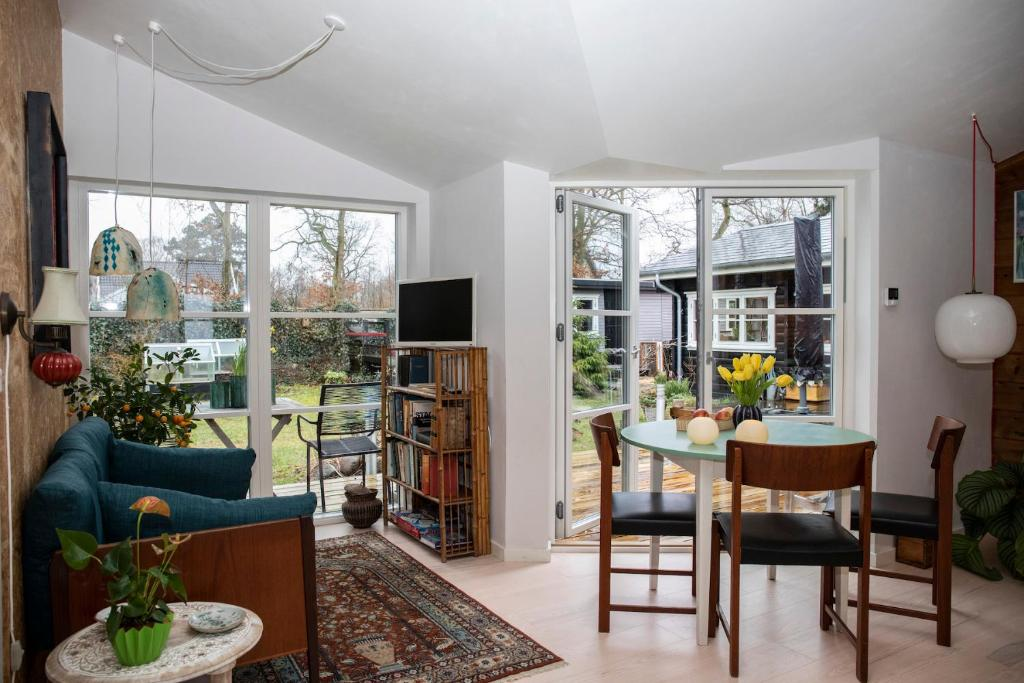
\includegraphics[width=\textwidth]{Kopenhagen/183496537.jpg}
        \caption{Unterkunft bei Kopenhagen}
        \label{fig:kopenhagen_unterkunft_1}
    \end{minipage}
    \hfill
    \begin{minipage}{0.48\textwidth}
        \centering
        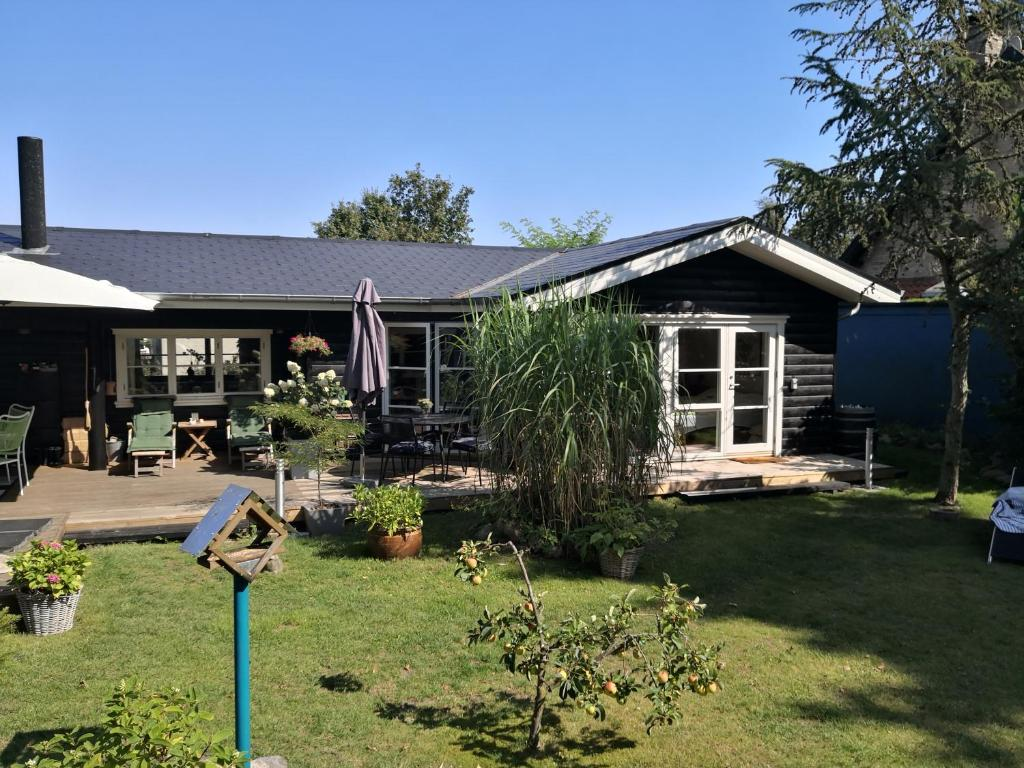
\includegraphics[width=\textwidth]{Kopenhagen/233219480.jpg}
        \caption{Zimmeransicht Kopenhagen}
        \label{fig:kopenhagen_unterkunft_2}
    \end{minipage}
\end{figure}


\subsection{In der Nähe von Göteborg}

In der Nähe von Göteborg übernachten wir zwei Nächte vom Do., 13.08.2026 bis Sa., 15.08.2026.

\textbf{Apartment Near Sea and Nature, Free Parking \& Cleaning}

\textit{Buchungsdetails:}
\begin{itemize}
\item Buchungs-Nr.: 5733.529.223
\item PIN-Code: 1106
\item Adresse: Lerduvevägen 4, 436 51 Göteborg, Schweden
\item Anreise: Do., 13.08.2026, 15:00--23:00 Uhr
\item Abreise: Sa., 15.08.2026, 08:00--12:00 Uhr
\item Übernachtungen: 2 Nächte
\item Personen: 2 Erwachsene
\item Unterkunft: Apartment mit 1 Schlafzimmer
\item Verpflegung: Keine Mahlzeit inbegriffen
\item Gesamtkosten: ca. 368 EUR / 4.050 SEK
\end{itemize}

\textit{Unterkunft und Leistungen:}
\begin{itemize}
\item Eigenes Badezimmer, Terrasse, Blick auf Garten und Berge
\item Küche mit Backofen, Herdplatte, Mikrowelle, Toaster, Spülmaschine und Wasserkocher
\item Waschmaschine, Bügeleisen, Kaffeemaschine, TV und Flachbild-TV
\item Sitzbereich, Essbereich, Schreibtisch, Safe und privater Eingang
\item Kostenfreies WLAN in allen Bereichen
\item Kostenfreie Privatparkplätze an der Unterkunft
\end{itemize}

\textit{Wichtige Hinweise:}
\begin{itemize}
\item In dieser Unterkunft sind keine Junggesellen- oder Junggesellinnenabschiede erlaubt.
\item Stornierung bis 10.08.2026, 23:59 Uhr kostenlos.
\item Ab 11.08.2026, 00:00 Uhr fallen Stornierungsgebühren von 2.025 SEK an.
\item Ab 14.08.2026, 00:00 Uhr fallen Stornierungsgebühren von 4.050 SEK an.
\item Eine Änderung der Reisedaten ist laut Bestätigung nicht möglich.
\item Die Stornierungsfristen gelten gemäß der Zeitzone der Unterkunft.
\end{itemize}

\textit{Kontaktdaten:}
\begin{itemize}
\item Telefon: +46 73 500 20 79
\item GPS-Koordinaten: N 057° 37.117, E 11° 57.002
\item Buchung online verwaltbar über: \url{https://your.booking.com}
\end{itemize}

\begin{figure}[H]
    \centering
    \begin{minipage}{0.48\textwidth}
        \centering
        
\includegraphics[width=\textwidth]{\detokenize{Göteborg/729899465.jpg}}
        \caption{Apartment bei Göteborg}
        \label{fig:goeteborg_apartment_1}
    \end{minipage}
    \hfill
    \begin{minipage}{0.48\textwidth}
        \centering
        
\includegraphics[width=\textwidth]{\detokenize{Göteborg/731736193.jpg}}
        \caption{Wohnbereich Göteborg}
        \label{fig:goeteborg_apartment_2}
    \end{minipage}
\end{figure}

\subsection{Blokhus}

\textbf{Ferienhaus „Amina" - 200m from the sea}

\textit{Buchungsdetails:}
\begin{itemize}
\item Buchungs-Nr.: 505926124704/1 (Interhome)
\item Referenz-Nr.: DK9492.769.1
\item Anreise: Sa., 15.08.2026, 16:00--00:00 Uhr
\item Abreise: Sa., 22.08.2026, bis 10:00 Uhr
\item Übernachtungen: 7 Nächte
\item Personen: 2 Erwachsene
\item Gesamtkosten: \mbox{1.633},00 EUR
\end{itemize}

\textit{Schlüsselübergabe und Anreisehinweise:}
\begin{itemize}
\item Schlüsselhalter: Sol og Strand NW Jutland
\item Adresse Schlüsselübergabe: Dahl Iversensvej 3, DK-9492 Blokhus
\item Kontakt Schlüsselhalter: +45 98 24 87 88, blokhus@sologstrand.dk
\item Schlüsselabholung über Schlüsselbox neben der Haustür hinter der halbhohen Mauer
\item Code der Schlüsselbox: 2560
\item Bei Anreise außerhalb der angegebenen Zeiten ist eine vorherige Bestätigung durch den Schlüsselhalter erforderlich.
\end{itemize}

\textit{Wichtige Hinweise zur Nutzung und Abreise:}
\begin{itemize}
\item Grundreinigung vor Abreise durch uns als Gäste erforderlich (u.a. Küche, Geschirr, Müll, Lebensmittelreste, Betten abziehen, besenreine Übergabe).
\item Schlüsselrückgabe am Abreisetag bis spätestens 10:00 Uhr; Abreisezeit vorab mit dem Schlüsselhalter abstimmen.
\item Nebenkosten (z.B. Kurtaxe oder Zusatzleistungen) werden vor Ort direkt abgerechnet.
\item Zahlungsregel für Nebenkosten vor Ort: Kartenzahlung bevorzugt, zusätzlich ausreichend Bargeld als Fallback mitführen.
\item Mängel sollen innerhalb von 48 Stunden gemeldet werden.
\item Maximalbelegung darf nicht überschritten werden.
\end{itemize}

\textit{Zahlungsstatus Interhome:}
\begin{itemize}
\item 30.12.2025: Abbuchung über 327,00 EUR per Kreditkarte
\item 20.07.2026: Abbuchung über 1.306,00 EUR per Kreditkarte
\end{itemize}

\textit{Unterkunft:}
\begin{itemize}
\item 3-Zimmer-Einfamilienhaus, 145 m², Baujahr 1919
\item 200 m vom Meer entfernt
\item Grundstück: \mbox{1.362} m²
\item 4 Sterne, geeignet für bis zu 5 Erwachsene
\item Ausstattung: Wohnzimmer mit TV, 2 Schlafzimmer mit Doppelbett, 1 Schlafzimmer mit Einzelbett
\item Vollausgestattete Küche (Backofen, Geschirrspüler, 4 Induktionskochplatten, Mikrowelle, Tiefkühler)
\item Dusche/WC, Meerblick
\item WLAN, Waschmaschine, Wäschetrockner
\item Grill, Parkplatz am Haus
\item Nichtraucher-Unterkunft, keine Haustiere
\end{itemize}

\textit{Lage und Umgebung:}
\begin{itemize}
\item Blokhus, bekannter Badeort mit 500 Einwohnern
\item 42 km nordwestlich von Aalborg, 75 km nordöstlich von Thisted
\item 5 km langer Sandstrand, flach abfallend, nur 50 m vom Ort entfernt
\item Aktivitäten: Surfen, 18-Loch-Golfplatz (4 km), Minigolf, Angeln, Wandern, Fahrradfahren
\item Infrastruktur: Supermarkt, Bäckerei, Restaurant, Bar, Wellnesszentrum
\item Kinderland Fårup Sommerland in 4 km Entfernung
\item Lebensmittelgeschäft in 2 km Entfernung
\end{itemize}

\begin{figure}[H]
    \centering
    \begin{minipage}{0.48\textwidth}
        \centering
        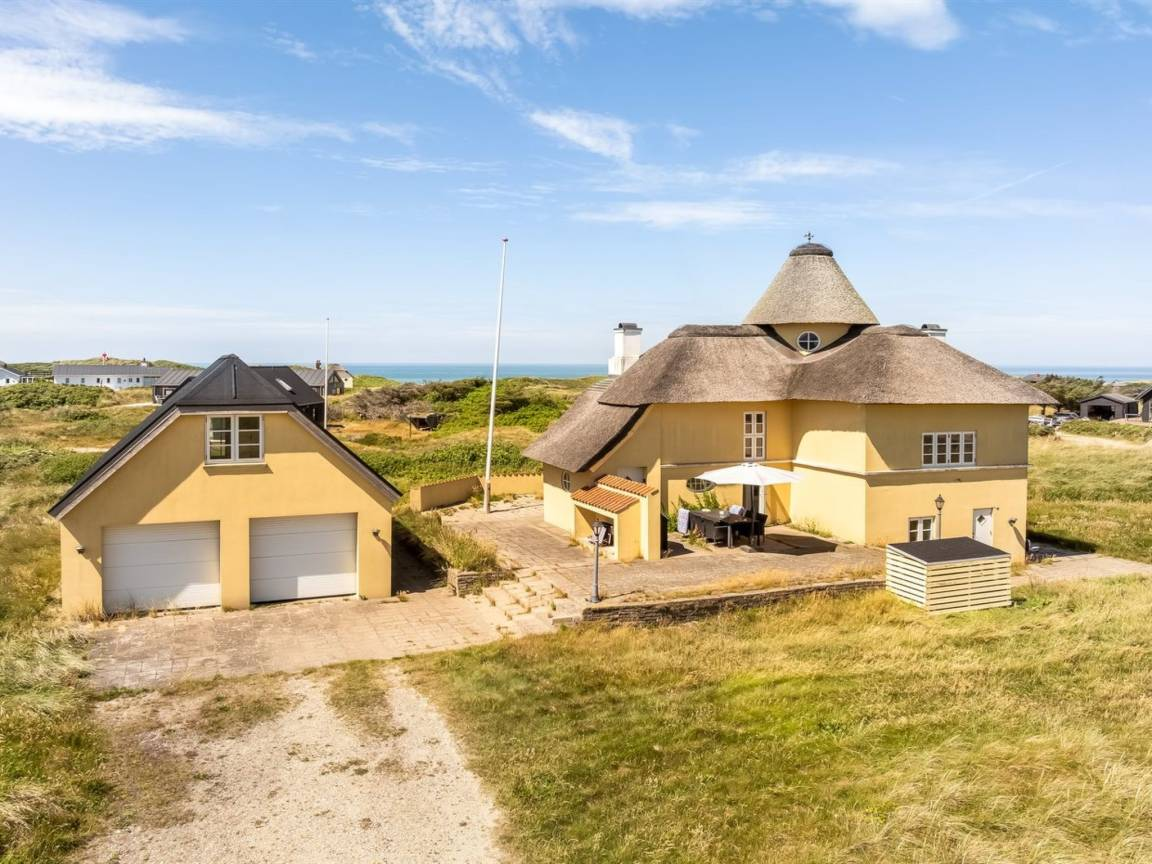
\includegraphics[width=\textwidth]{Blokhus/House Amina - Blokhus.jpg}
        \caption{Ferienhaus Amina in Blokhus}
        \label{fig:amina_haus}
    \end{minipage}
    \hfill
    \begin{minipage}{0.48\textwidth}
        \centering
        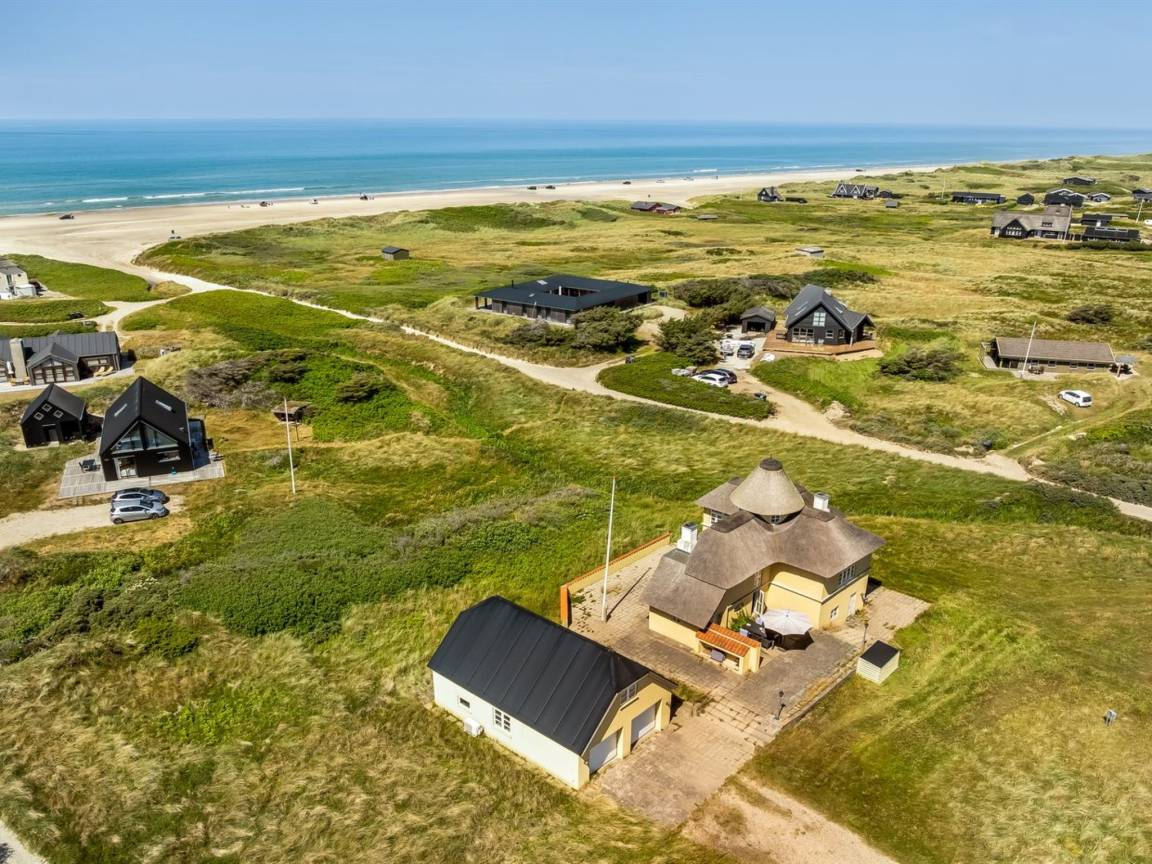
\includegraphics[width=\textwidth]{Blokhus/House Amina - Meeresblick.jpg}
        \caption{Meerblick vom Ferienhaus Amina}
        \label{fig:amina_meeresblick}
    \end{minipage}
\end{figure}


% Zeitplan
\section{Zeitplan}
Reisetage (An-/Abreise und Fahrten zwischen Unterkünften) sind separat von Urlaubstagen mit Aktivitäten gekennzeichnet.

\begin{table}[H] % Erzwungene Platzierung
\centering
\begin{tabular}{|l|l|l|l|}
\hline
\textbf{Datum} & \textbf{Ort / Abschnitt} & \textbf{Tagestyp} & \textbf{Planung} \\
\hline
08.08. & Weinheim $\rightarrow$ Lübeck & Reisetag & Anreise mit dem Auto, Check-in Lübeck \\
09.08. & Lübeck & Urlaubstag & Altstadt, Holstentor, Hafen/Travemünde \\
10.08. & Lübeck $\rightarrow$ Kopenhagen & Reisetag & Check-out, Fahrt nach Kopenhagen, Check-in \\
11.08. & Kopenhagen & Urlaubstag & Stadttag und Sehenswürdigkeiten \\
12.08. & Kopenhagen & Urlaubstag & Reservetag für Aktivitäten/Ausflüge \\
13.08. & Kopenhagen $\rightarrow$ Göteborg & Reisetag & Check-out, Fahrt nach Göteborg, Check-in \\
14.08. & Göteborg & Urlaubstag & Stadtbesichtigung / Museumsbesuch \\
15.08. & Göteborg $\rightarrow$ Blokhus & Reisetag & Check-out, Fähr-/Autofahrt, Check-in Blokhus \\
16.08. & Blokhus & Urlaubstag & Strand und Erholung \\
17.08. & Blokhus & Urlaubstag & Freier Urlaubstag / Ausflug \\
18.08. & Blokhus & Urlaubstag & Freier Urlaubstag / Aktivitäten \\
19.08. & Blokhus & Urlaubstag & Freier Urlaubstag / Aktivitäten \\
20.08. & Blokhus & Urlaubstag & Freier Urlaubstag / Aktivitäten \\
21.08. & Blokhus & Urlaubstag & Letzter voller Urlaubstag \\
22.08. & Blokhus $\rightarrow$ Weinheim & Reisetag & Rückreise ab 09:00, Haus bis 10:00 freigeben \\
\hline
\end{tabular}
\caption{Zeitplan mit Unterscheidung zwischen Reise- und Urlaubstagen.}
\label{tab:Zeitplan}
\end{table}

\subsection*{Checkliste offene Ablaufpunkte}
\begin{itemize}
\item [x] Verbindliche Abfahrtszeit der Fähre Göteborg $\rightarrow$ Frederikshavn am 15.08. festgelegt (09:05--12:35, Stena Danica; Check-in 30 Minuten vorher).
\item [x] Konkrete Startzeit der Rückreise am 22.08. festgelegt (Abfahrt 09:00, Haus bis 10:00 freigeben).
\item [x] Pausenplanung für die Fahrten definiert (zusätzliche Ladestopps: 30 Minuten je 350--400 km).
\item [x] Verspätungsregel festgelegt (ab 45 Minuten erwarteter Verspätung Unterkunft telefonisch informieren).
\item [x] Regel für Nebenkosten vor Ort festgelegt (Kartenzahlung bevorzugt, Bargeld als Fallback mitführen).
\item [x] Gesamtreisezeit im Dokument vereinheitlicht (reine Fahrzeit 29h 47min zzgl. Ladepuffer).
\end{itemize}

% Budget
\section{Budget}
\begin{table}[H] % Erzwungene Platzierung
\centering
\begin{tabular}{|l|r|}
\hline
\textbf{Posten} & \textbf{Kosten (EUR)} \\
\hline
Hotel IV Jahreszeiten Lübeck & 304,65  \\
Unterkunft bei Kopenhagen & 278,00 \\
Unterkunft bei Göteborg & 368,00 \\
Maut (E20) Öresundbrücke & 53,00  \\
Fähre Göteborg - Frederikshavn & 200,00 \\
Unterkunft in Blokhus & 1.633,00  \\
Verpflegung & 200,00 \\
\hline
\textbf{Gesamt} & \textbf{3.036,65} \\
\hline
\end{tabular}
\caption{Budgetübersicht der Reise.}
\label{tab:Budget}
\end{table}

% Tabelle mit den wichtigsten Reisedaten
\section{Reisedaten}

\begin{table}[H] % Erzwungene Platzierung
\centering
\begin{tabular}{|l|l|r|l|}
\hline
\textbf{Reiseziel (Ort)} & \textbf{Fahrttag} & \textbf{Kilometer} & \textbf{Fahrtzeit} \\
\hline
Lübeck & Sa., 08.08.2026 & 604 & 6h 13min \\
Kopenhagen & Mo., 10.08.2026 & 273 & 4h 11min \\
Göteborg & Do., 13.08.2026 & 313 & 3h 31min \\
Blokhus & Sa., 15.08.2026 & 176 & 5h 16min \\
Weinheim & Sa., 22.08.2026 & 1.035 & 10h 36min \\
\hline
\textbf{Gesamt} & & \textbf{\mbox{2.401}} & \textbf{29h 47min} \\
\hline
\end{tabular}
\caption{Übersicht der wichtigsten Reisedaten.}
\label{tab:Reisedaten}
\end{table}

\end{document}